\documentclass[a4paper]{article}
    \usepackage[UTF8]{ctex}
    \usepackage{amsmath,amsthm,amssymb}

    \usepackage{minted}
    \usepackage{xcolor}
    \usepackage[colorlinks,linkcolor=black]{hyperref}
    \usepackage[margin=1in]{geometry}
    \usepackage{caption}
    \usepackage{graphicx}
    \usepackage{subfigure}
    \usepackage{float}
    \usepackage{fontspec}
    \usepackage{booktabs}
    \setmainfont{Times New Roman}
    \setmonofont{Consolas}
    \definecolor{bg}{rgb}{0.9,0.9,0.9}
    \usemintedstyle{manni}
    \setminted{
    linenos,
    autogobble,
    breaklines,
    breakautoindent,
    bgcolor=bg,
    numberblanklines=false,
    }

\begin{document}
    \tableofcontents
    \newpage
    \section{实验介绍}
        \subsection{实验内容}
对dataset文件夹中的图片进行Canny边缘检测,并与OpenCV库中自带Canny检测结果进行对比.

可选取不同梯度幅值算子与阈值获得更优的检测性能.
        \subsection{实验环境}
操作系统: Ubuntu 18.04 LTS

Python版本: 3.7

NumPy: 1.14.5

OpenCV-Python: 3.4.3.18
    \newpage
    \section{实验过程}
        \subsection{Canny边缘检测原理}
Canny边缘检测是一种目前被广泛使用的图像边缘检测算法,于1986年由John F. Canny提出.Canny边缘检测算法是一种多阶段算法,
可以分为以下5个步骤:

1.使用高斯滤波器,以平滑图像,滤除噪声.

2.计算图像中每个像素点的梯度(包含强度和方向).

3.应用非极大值抑制,消除边缘检测带来的杂散响应.

4.应用双阈值算法来确定真实的边缘,潜在的边缘,以及非边缘.

5.抑制孤立的弱边缘最终完成边缘检测.


    \subsection{灰度化及高斯滤波}
    \label{gaussian}
对于一张彩色图片,以RGB格式读入之后,需要将其进行灰度化处理. 为了方便调节灰度化的具体参数,自行编写的处理函数如下:
\begin{minted}{python}
def rgb_to_grayscale(rgb_img):
    ratios = [0.114, 0.587, 0.299]
    result = np.zeros(rgb_img.shape[:-1], dtype="float32")
    for i in range(3):
        result += ratios[i] * rgb_img[:, :, i]
    result = result.astype("uint8")
    return result
\end{minted}

在经过灰度化处理之后,为了滤除图像中的噪声,避免对后续边缘检测造成影响,可采用高斯滤波的方法,平滑图像.大小为$(2k+1)*(2k+1)$的高斯滤波
器核的生成方式如下:

$$K_{ij} = \frac{1}{2\pi \sigma^{2}}e^{-\frac{(i-(k+1))^2 + (j-(j+1))^2}{2\sigma^2}},1\leq i,j \leq 2k+1$$

事实上,上式即为二维正态分布概率密度公式.但在生成了高斯滤波器核之后,还需要对其进行归一化处理,使其中元素之和为1.完整代码如下:

\begin{minted}{python}
def get_gaussian_kernel(size=3, sigma=1):
    kernel = np.zeros((size, size))
    k = int((size-1)/2)
    for x in range(-k, k+1):
        for y in range(-k, k+1):
            kernel[k+x][k+y] = np.exp(-(x*x+y*y)/(2*sigma*sigma)) / (2*np.pi*sigma*sigma)
    kernel = kernel / np.sum(kernel)
    return kernel
\end{minted}

在得到高斯核之后,可调用OpenCV函数,对图像进行卷积处理:
\begin{minted}{python}
gaussian_blur_img = cv2.filter2D(img, -1, kernel)
\end{minted}

需要注意的是,高斯卷积核大小的选择将影响Canny检测器的性能:尺寸越大,Canny检测器对噪声的敏感度就越低,
但是边缘检测的定位误差也将略有增加.

        \subsection{计算梯度}
关于图像灰度值的梯度,可使用一阶有限差分来进行近似计算.常见的梯度算子有Roberts算子,Sobel算子,Prewitt算子等.不同的梯度算子有着
不同的效果,影响Canny边缘检测算法的最终结果.在本次实验中,我选择了Sobel算子.

Sobel算子的x,y方向卷积模板为:
$$
s_x = 
\begin{pmatrix}
-1 & 0 & 1\\
-2 & 0 & 2\\ 
-1 & 0 & 1\\
\end{pmatrix} ,
s_y =
\begin{pmatrix}
1 & 2 & 1\\
0 & 0 & 0 \\
-1 & -2 & -1\\
\end{pmatrix} 
$$

对每个像素点,分别在x方向和y方向进行卷积之后,得到梯度的x方向和y方向上的分量$g_x,g_y$.则梯度的强度和方向定义为:
$$M(i,j) = \sqrt{g_{x}^{2} + g_{y}^{2}}$$
$$\theta(i,j) = \arctan{\frac{g_y}{g_x}}$$

需要注意的是,考虑到梯度的方向可能为$\pm \pi/2$,此时$g_x =0$,为避免除法出错,需要将计算梯度方向的公式略作修改:
$$\theta(i,j) = \arctan{\frac{g_y}{g_x + \epsilon}}$$

故完整的代码如下:
\begin{minted}{python}
def sobel(img):
    result = np.zeros_like(img)
    direction = np.zeros_like(img)
    width, height = img.shape
    s_y = np.array([
        [-1, 0, 1],
        [-2, 0, 2],
        [-1, 0, 1], ])
    s_x = np.array([
        [1, 2, 1],
        [0, 0, 0],
        [-1, -2, -1], ])
    for i in range(1, width-1):
        for j in range(1, height-1):
            x = np.sum(img[i-1:i+2, j-1:j+2] * s_x)
            y = np.sum(img[i-1:i+2, j-1:j+2] * s_y)
            result[i][j] = np.sqrt(x * x + y * y)
            direction[i][j] = np.arctan(y/(x+1e-5))
    result = result.astype("uint8")
    return result, direction
\end{minted}
        \subsection{非极大值抑制}
在Canny边缘检测算法中,需要抑制那些梯度强度非极大的像素点.

\begin{figure}[H]
\centering
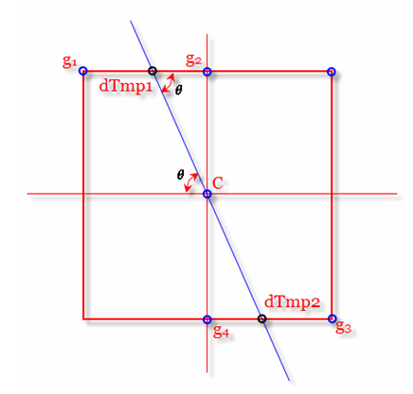
\includegraphics[width=.6\textwidth]{img/nms.png}
\caption{插值法}
\end{figure}

如图所示,对于点C,沿着其梯度方向,与图像的像素网格产生了两个最近的交点$dTmp1$和$dTmp2$,
为确保C是梯度的极大值点,需要满足C点的梯度强度比这两点都要大,否则就将其抑制.而由于$dTmp1,dTmp2$这两点并非图像本身的
像素点,其梯度值只能通过插值法得到.

简便起见,本次实验中我采用了线性插值法.以$dTmp1$点为例,其梯度值介于$g_1$和$g_2$之间,则根据$dTmp1$到两者的距离比例,
计算出该点的梯度值即可.

在程序实现中,根据梯度方向不同,分为了$|\theta|<\pi/4$和$|\theta|\geq \pi/4$两类进行处理,具体如下

\begin{minted}{python}
def non_maximum_suppression(gradient, direction):
    result = np.zeros_like(gradient)
    width, height = gradient.shape
    for i in range(1, width-1):
        for j in range(1, height - 1):
            if -np.pi/4 < direction[i][j] < np.pi/4:
                x1, y1 = i + 1, j + np.tan(direction[i][j])
                x2, y2 = i - 1, j - np.tan(direction[i][j])
                temp1 = (y1 - int(y1))*gradient[x1][min(height-1, int(y1)+1)]
                    + (int(y1) + 1 - y1)*gradient[x1][int(y1)]
                temp2 = (y2 - int(y2))*gradient[x2][min(height-1, int(y2)+1)]
                    + (int(y2) + 1 - y2)*gradient[x2][int(y2)]
            else:
                x1, y1 = i + 1/np.tan(direction[i][j]), j + 1
                x2, y2 = i - 1/np.tan(direction[i][j]), j - 1
                temp1 = (x1 - int(x1))*gradient[min(width-1, int(x1)+1)][y1] 
                    + (int(x1) + 1 - x1)*gradient[int(x1)][y1]
                temp2 = (x2 - int(x2))*gradient[min(width-1, int(x2)+1)][y2]
                    + (int(x2) + 1 - x2)*gradient[int(x2)][y2]
            if(gradient[i][j] >= temp1 and gradient[i][j] >= temp2):
                result[i][j] = gradient[i][j]
    return result
\end{minted}

        \subsection{双阈值检测}
        \label{double_threshold}
在施加非极大值抑制之后,为了减少假边缘,Canny边缘检测算法采取了双阈值检测的做法.即设定高阈值和低阈值,对于每一个像素点的梯度强度,
如果高于高阈值,则确定其为图像的边缘像素点;如果低于低阈值,则认为其不为边缘像素点,将其抑制;如果处于高低阈值之间,则将其标记为弱边缘像素点,
留待进一步处理.

在程序实现中,为了方便,将弱边缘像素点的值设置为1,强边缘像素点的值设置为255.

\begin{minted}{python}
def double_threshold(img, low, high):
    result = np.zeros_like(img)
    width, height = img.shape
    for i in range(0, width):
        for j in range(0, height):
            result[i][j] = 254*(img[i][j] >= high) + 1*(img[i][j] >= low)
    return result
\end{minted}

    \subsection{抑制孤立弱边缘点}
弱边缘点可能是真的边缘,也可能是由噪声引起的误差.对于前者,我们需要保留,而后者,则需要将其抑制.Canny边缘检测算法认为,
如果一个弱边缘点周围的8个领域像素中存在强边缘点,那么它是一个边缘像素点,否则便是需要被抑制的噪声.

在我的程序实现中,为了更好的处理那些不确定是否为边缘的点,多次尝试,直到完全确定其不为边缘点为止.

\begin{minted}{python}
def track_edge(img):
    result = np.zeros_like(img)
    uncertain_points = list()
    width, height = img.shape
    for i in range(1, width-1):
        for j in range(1, height-1):
            if img[i][j] == 255:
                result[i][j] = 255
            elif img[i][j] == 1:
                result[i][j] = 0
                doubt = False
                for x in range(i-1, i+2):
                    for y in range(j-1, j+2):
                        if img[x][y] == 255:
                            result[i][j] = 255
                        elif img[x][y] == 1:
                            doubt = True
                if(result[i][j] == 0 and doubt):
                    uncertain_points.append((i, j))
    prev_len = 0
    while(prev_len != len(uncertain_points)):
        prev_len = len(uncertain_points)
        print(prev_len)
        still_uncertain = list()
        for point in uncertain_points:
            for x in range(point[0]-1, point[0]+2):
                for y in range(point[1]-1, point[1]+2):
                    if result[x][y] == 255:
                        result[point[0]][point[1]] = 255
            if result[point[0]][point[1]] == 0:
                still_uncertain.append(point)
        uncertain_points = still_uncertain
    return result
\end{minted}

\newpage

\section{检测效果与参数设置}
    \subsection{完整检测流程}
图\ref{Fig.lable}展示了Canny边缘检测的完整流程,并给出了OpenCV库中的Canny()函数的处理结果,以供对比.
\begin{figure}[H]
\centering
\subfigure[原始图片]{
\label{Fig.sub.1}
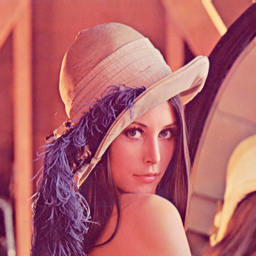
\includegraphics[width=0.2\textwidth]{img/size3sigma1low50high100/0.png}}
\subfigure[灰度图片]{
\label{Fig.sub.2}
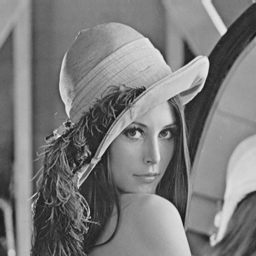
\includegraphics[width=0.2\textwidth]{img/size3sigma1low50high100/1.png}}
\subfigure[高斯滤波]{
\label{Fig.sub.2}
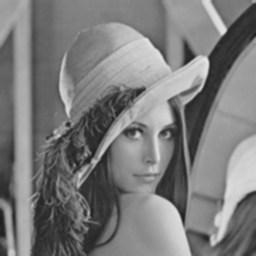
\includegraphics[width=0.2\textwidth]{img/size3sigma1low50high100/2.png}}
\subfigure[计算图像梯度]{
\label{Fig.sub.2}
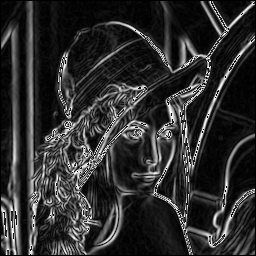
\includegraphics[width=0.2\textwidth]{img/size3sigma1low50high100/3.png}}
\subfigure[非极大值抑制]{
\label{Fig.sub.2}
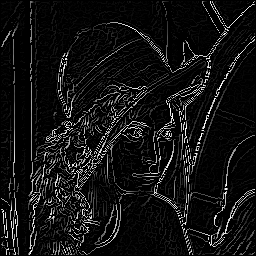
\includegraphics[width=0.2\textwidth]{img/size3sigma1low50high100/4.png}}
\subfigure[双阈值检测]{
\label{Fig.sub.2}
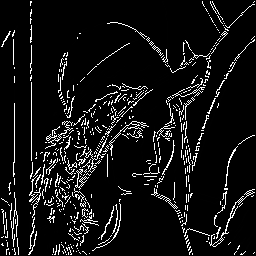
\includegraphics[width=0.2\textwidth]{img/size3sigma1low50high100/5.png}}
\subfigure[抑制孤立弱边缘点(最终结果)]{
\label{Fig.sub.2}
\includegraphics[width=0.2\textwidth]{img/size3sigma1low50high100/final.png}}
\subfigure[OpenCV.Canny函数处理结果]{
\label{Fig.sub.2}
\includegraphics[width=0.2\textwidth]{img/size3sigma1low50high100/opencv.png}}
\caption{Canny边缘检测流程(size=3,sigma=1,low=50,high=100)}
\label{Fig.lable}
\end{figure}
    \subsection{高斯核参数}
根据\ref{gaussian},可知在进行高斯滤波处理时,主要有两个可以调节的参数:高斯核的尺寸(size)与高斯分布函数的标准差(sigma).

直观上分析,当高斯核的尺寸增大时,高斯模糊的效果增强,从而能够更好的抵御图像中的噪声,但也不可避免地会失去一部分细节,从而导致最终的检测结果
精度下降;而当标准差增大时,高斯分布趋于平缓,从而同样的使得高斯模糊的效果增强.

按不同的高斯滤波参数进行实验,得到的结果如组图\ref{guassian_parameters}所示(各组实验的low,high均为50,100),分析边缘检测的效果,
与上述直观的想法基本一致.同时也选定了较优的参数设定:size=3,sigma=1.

\begin{figure}[H]
\centering
\subfigure[高斯滤波(size=5,sigma=1)]{
\includegraphics[width=0.2\textwidth]{img/gaussian/size5sigma1/1.png}}
\subfigure[最终结果(size=5,sigma=1)]{
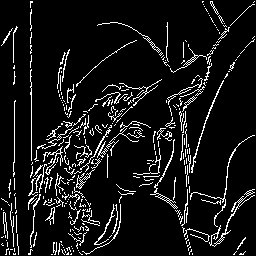
\includegraphics[width=0.2\textwidth]{img/gaussian/size5sigma1/2.png}}
\subfigure[高斯滤波(size=3,sigma=1)]{
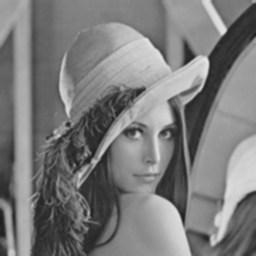
\includegraphics[width=0.2\textwidth]{img/gaussian/size3sigma1/1.png}}
\subfigure[最终结果(size=3,sigma=1)]{
\includegraphics[width=0.2\textwidth]{img/gaussian/size3sigma1/2.png}}
\subfigure[高斯滤波(size=7,sigma=1)]{
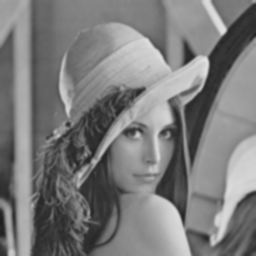
\includegraphics[width=0.2\textwidth]{img/gaussian/size7sigma1/1.png}}
\subfigure[最终结果(size=7,sigma=1)]{
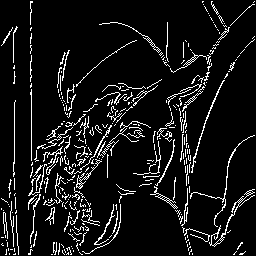
\includegraphics[width=0.2\textwidth]{img/gaussian/size7sigma1/2.png}}
\subfigure[高斯滤波(size=5,sigma=2)]{
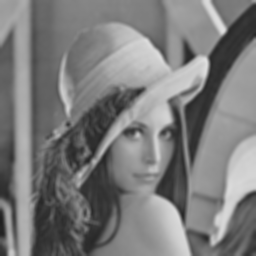
\includegraphics[width=0.2\textwidth]{img/gaussian/size5sigma2/1.png}}
\subfigure[最终结果(size=5,sigma=2)]{
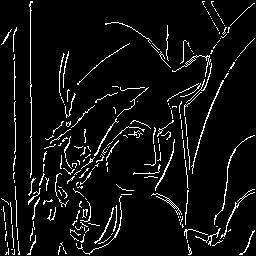
\includegraphics[width=0.2\textwidth]{img/gaussian/size5sigma2/2.png}}
\subfigure[高斯滤波(size=5,sigma=0.5)]{
\includegraphics[width=0.2\textwidth]{img/gaussian/size5sigma0.5/1.png}}
\subfigure[最终结果(size=5,sigma=0.5)]{
\includegraphics[width=0.2\textwidth]{img/gaussian/size5sigma0.5/2.png}}
\caption{Canny边缘检测效果与高斯滤波参数}
\label{guassian_parameters}
\end{figure}
    \subsection{双阈值检测参数}
由\ref{double_threshold}中的原理可知,高低阈值影响着Canny算法对图像中噪声与细节的相互取舍,不同的阈值必然会产生不同的
边缘检测效果.

依旧是先从直观上进行分析:若高阈值和低阈值都设定的很高,那么会失去很多细节;若高阈值和低阈值都设定的很低,那么会受到噪声的极大干扰,
最终产生的边缘将是很不平滑的;若高阈值很高,低阈值很低,那么大多数点将标记为弱边缘点,依赖于最后一步的孤立弱边缘点抑制,很可能导致
边缘不完整;若高阈值很低,低阈值很高,那么仅产生很少的弱边缘点,Canny算法发生了退化,不能充分发挥其效果.

按不同的阈值参数进行实验,得到的结果如组图\ref{double_parameters}所示(各组实验中size,sigma均为3,1),
分析结果,基本上与上述直观分析相符合.同时也发现,low=50,high=100是一组相对较好的阈值设定.
\begin{figure}[H]
\centering
\subfigure[双阈值检测(low=25,high=100)]{
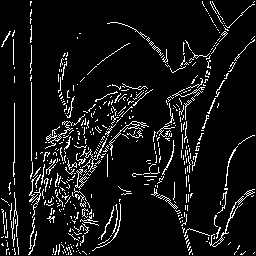
\includegraphics[width=0.2\textwidth]{img/double/low25high100/1.png}}
\subfigure[最终结果(low=25,high=100)]{
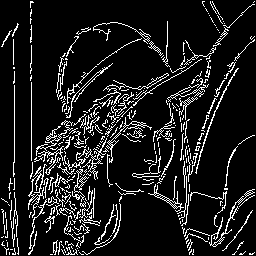
\includegraphics[width=0.2\textwidth]{img/double/low25high100/2.png}}
\subfigure[双阈值检测(low=50,high=100)]{
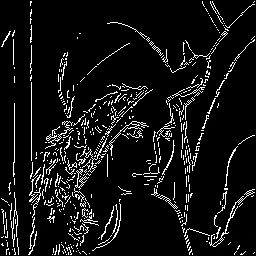
\includegraphics[width=0.2\textwidth]{img/double/low50high100/1.png}}
\subfigure[最终结果(low=50,high=100)]{
\includegraphics[width=0.2\textwidth]{img/double/low50high100/2.png}}
\subfigure[双阈值检测(low=50,high=150)]{
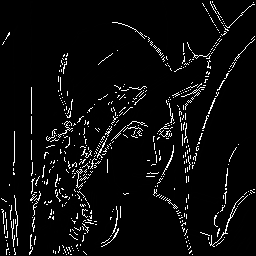
\includegraphics[width=0.2\textwidth]{img/double/low50high150/1.png}}
\subfigure[最终结果(low=50,high=150)]{
\includegraphics[width=0.2\textwidth]{img/double/low50high150/2.png}}
\subfigure[双阈值检测(low=50,high=200)]{
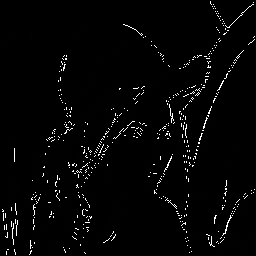
\includegraphics[width=0.2\textwidth]{img/double/low50high200/1.png}}
\subfigure[最终结果(low=50,high=200)]{
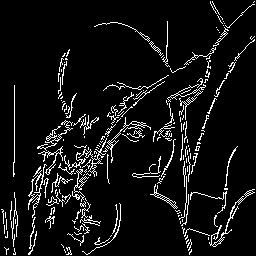
\includegraphics[width=0.2\textwidth]{img/double/low50high200/2.png}}
\subfigure[双阈值检测(low=100,high=150)]{
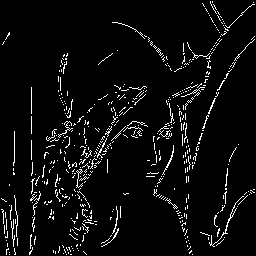
\includegraphics[width=0.2\textwidth]{img/double/low100high150/1.png}}
\subfigure[最终结果(low=100,high=150)]{
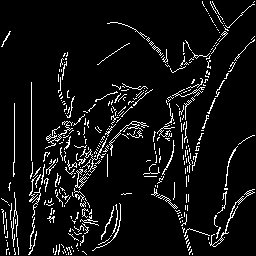
\includegraphics[width=0.2\textwidth]{img/double/low100high150/2.png}}
\subfigure[双阈值检测(low=100,high=200)]{
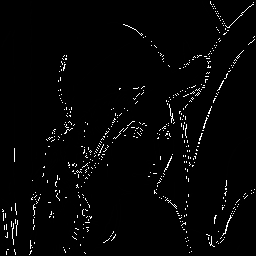
\includegraphics[width=0.2\textwidth]{img/double/low100high200/1.png}}
\subfigure[最终结果(low=100,high=200)]{
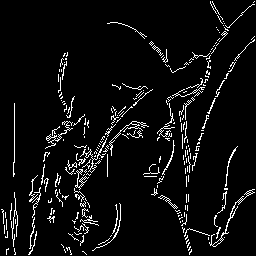
\includegraphics[width=0.2\textwidth]{img/double/low100high200/2.png}}
\caption{Canny边缘检测效果与双阈值参数}
\label{double_parameters}
\end{figure}
\newpage
\section{总结与分析}
本次实验中,我实现了基本的Canny边缘检测算法,并探索设定了其中的部分参数,以取得更好的边缘检测效果.在这个过程中,我对图像处理
的许多概念有了较为清晰的认知:譬如滤波,噪声处理,卷积等.

但在我看来,不可否认Canny算法能够比较好的实现图像的边缘检测,但其效果依赖于对具体图像的参数设定,一旦参数设定不当,
其效果远不能使人满意.而近年来的计算机视觉领域不断发展,带来了许多新的基于深度学习的图像处理方法,取得了更好的效果,
或许将来能够真正地基于内容对图像进行边缘检测,而非机械地基于图像特征处理.
\end{document}
